\documentclass[
	10pt,
	classe=$2^{de}$,
]{coursclass}

\title{Cours chapitre 1}
\author{Règles de calcul}
\date{}

\begin{document}

\maketitle

\setcounter{section}{2}
\section{Résolution d’équations et d’inéquations}

\begin{propriete}[Résolution d'équations]
	Si on effectue une \textit{même opération de base} (addition, soustraction, multiplication, division), en excluant la division par $0$, des \textbf{deux côtés de l'équation}, on obtient une équation équivalente (les solutions restent les mêmes).
\end{propriete}

\begin{exemple}
	\begin{align*}
		3x + 7 & = x + 15 &                           \\
		3x     & = x + 8  & \text{(on soustrait 7)}   \\
		2x     & = 8      & \text{(on soustrait $x$)} \\
		x      & = 4      & \text{(on divise par 2)}
	\end{align*}
\end{exemple}

\begin{propriete}[Résolution d'inéquations]
	Les mêmes règles que pour la résolution d'équation s'appliquent, \textbf{SAUF} :

	Si on effectue une multiplication ou une division par un nombre \textbf{strictement négatif} des deux côtés de l’inéquation, on obtient une inéquation équivalente (qui a les mêmes solutions) \textbf{à condition de changer le signe de l’inéquation} (inférieur devient supérieur ou inversement).
\end{propriete}

\begin{exemple}
	\begin{align*}
		-x + 2 & ≤ x + 6 &                                                                 \\
		-x     & ≤ x + 4 & \text{(on soustrait 2)}                                         \\
		-2x    & ≤ 4     & \text{(on soustrait $x$)}                                       \\
		x      & ≥ -2    & \text{(on divise par $-2$ : le signe de l'inéquation change !)} \\
	\end{align*}
\end{exemple}

\section{Valeur absolue et distance}

\begin{definition}[Valeur absolue]
	Si $x$ est un nombre négatif, on note $|x|$ et on appelle \textbf{valeur absolue} de $x$ la distance à zéro de $x$.

	C'est-à-dire :
	\begin{itemize}
		\item Si $x ≥ 0$, $|x| = x$.
		\item Si $x < 0$, $|x| = -x$.
	\end{itemize}
\end{definition}

\begin{exemple}
	\begin{align*}
		|2| & = 2 & |5,3| & = 5,3 & |-9| & = 9 & |-7,1| & = 7,1
	\end{align*}
\end{exemple}

\begin{definition}[distance sur une droite graduée]
	Soient $A$ un point d'abscisse $a$, et $B$ un point d'abscisse $b$, positionés sur une droite graduée.

	Alors la distance entre $A$ et $B$ est : $|a - b|$.
\end{definition}

\begin{propriete}[Équation avec une valeur absolue]
	Soit $A$ un point de la droite graduée d'abscisse $a$, et $d$ un nombre positif.

	Résoudre l'équation $|x - a| = d$ revient à trouver tous les points de la droite à distance $d$ du point $A$.
\end{propriete}

\begin{exemple}
	\begin{center}
		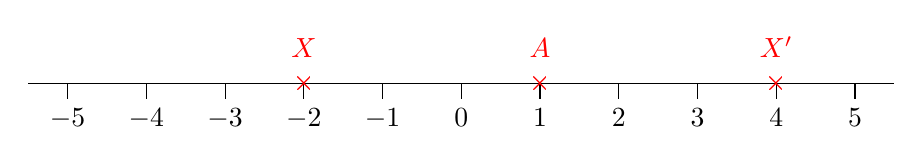
\begin{tikzpicture}
			\draw[\myArrow] (-5.5,0) -- (5.5,0);
			\foreach \x in {-5,...,5} {
					\draw (\x,0) -- ++(0,-0.2) node[below] {$\x$};
				}
			\foreach \p/\x in {A/1,X/-2,X'/4} {
					\node[red] at (\x,0) {×};
					\node[red,above] at (\x,0.2) {$\p$};
				}
		\end{tikzpicture}
	\end{center}

	Sur la droite ci-dessus, le point $A$ a pour abscisse $1$.

	Les points $X$ et $X'$ sont les deux points à distance $3$ du point $A$.

	Ainsi les solutions de l'équation $|x-1| = 3$ sont \squared{$x = -2$} et \squared{$x = 4$}.
\end{exemple}

\end{document}